\chapter{UI (optionale Erläuterung)}
\section{Frontend-Lobby}
\label{chap:frontend}

Die \textit{Lobby} bildet den Einstiegspunkt für die Spieler und ist der zentrale Bestandteil des Frontends. 
Sie wurde mit dem Framework \textbf{Angular} umgesetzt und mit \textbf{Bootstrap} für ein modernes, responsives Design gestaltet. 
Die in Abbildung~\ref{fig:frontend_lobby} dargestellte Oberfläche ermöglicht den Login, die Serverauswahl sowie die Anzeige von Spielstatistiken.

\begin{figure}[h!]
  \centering
  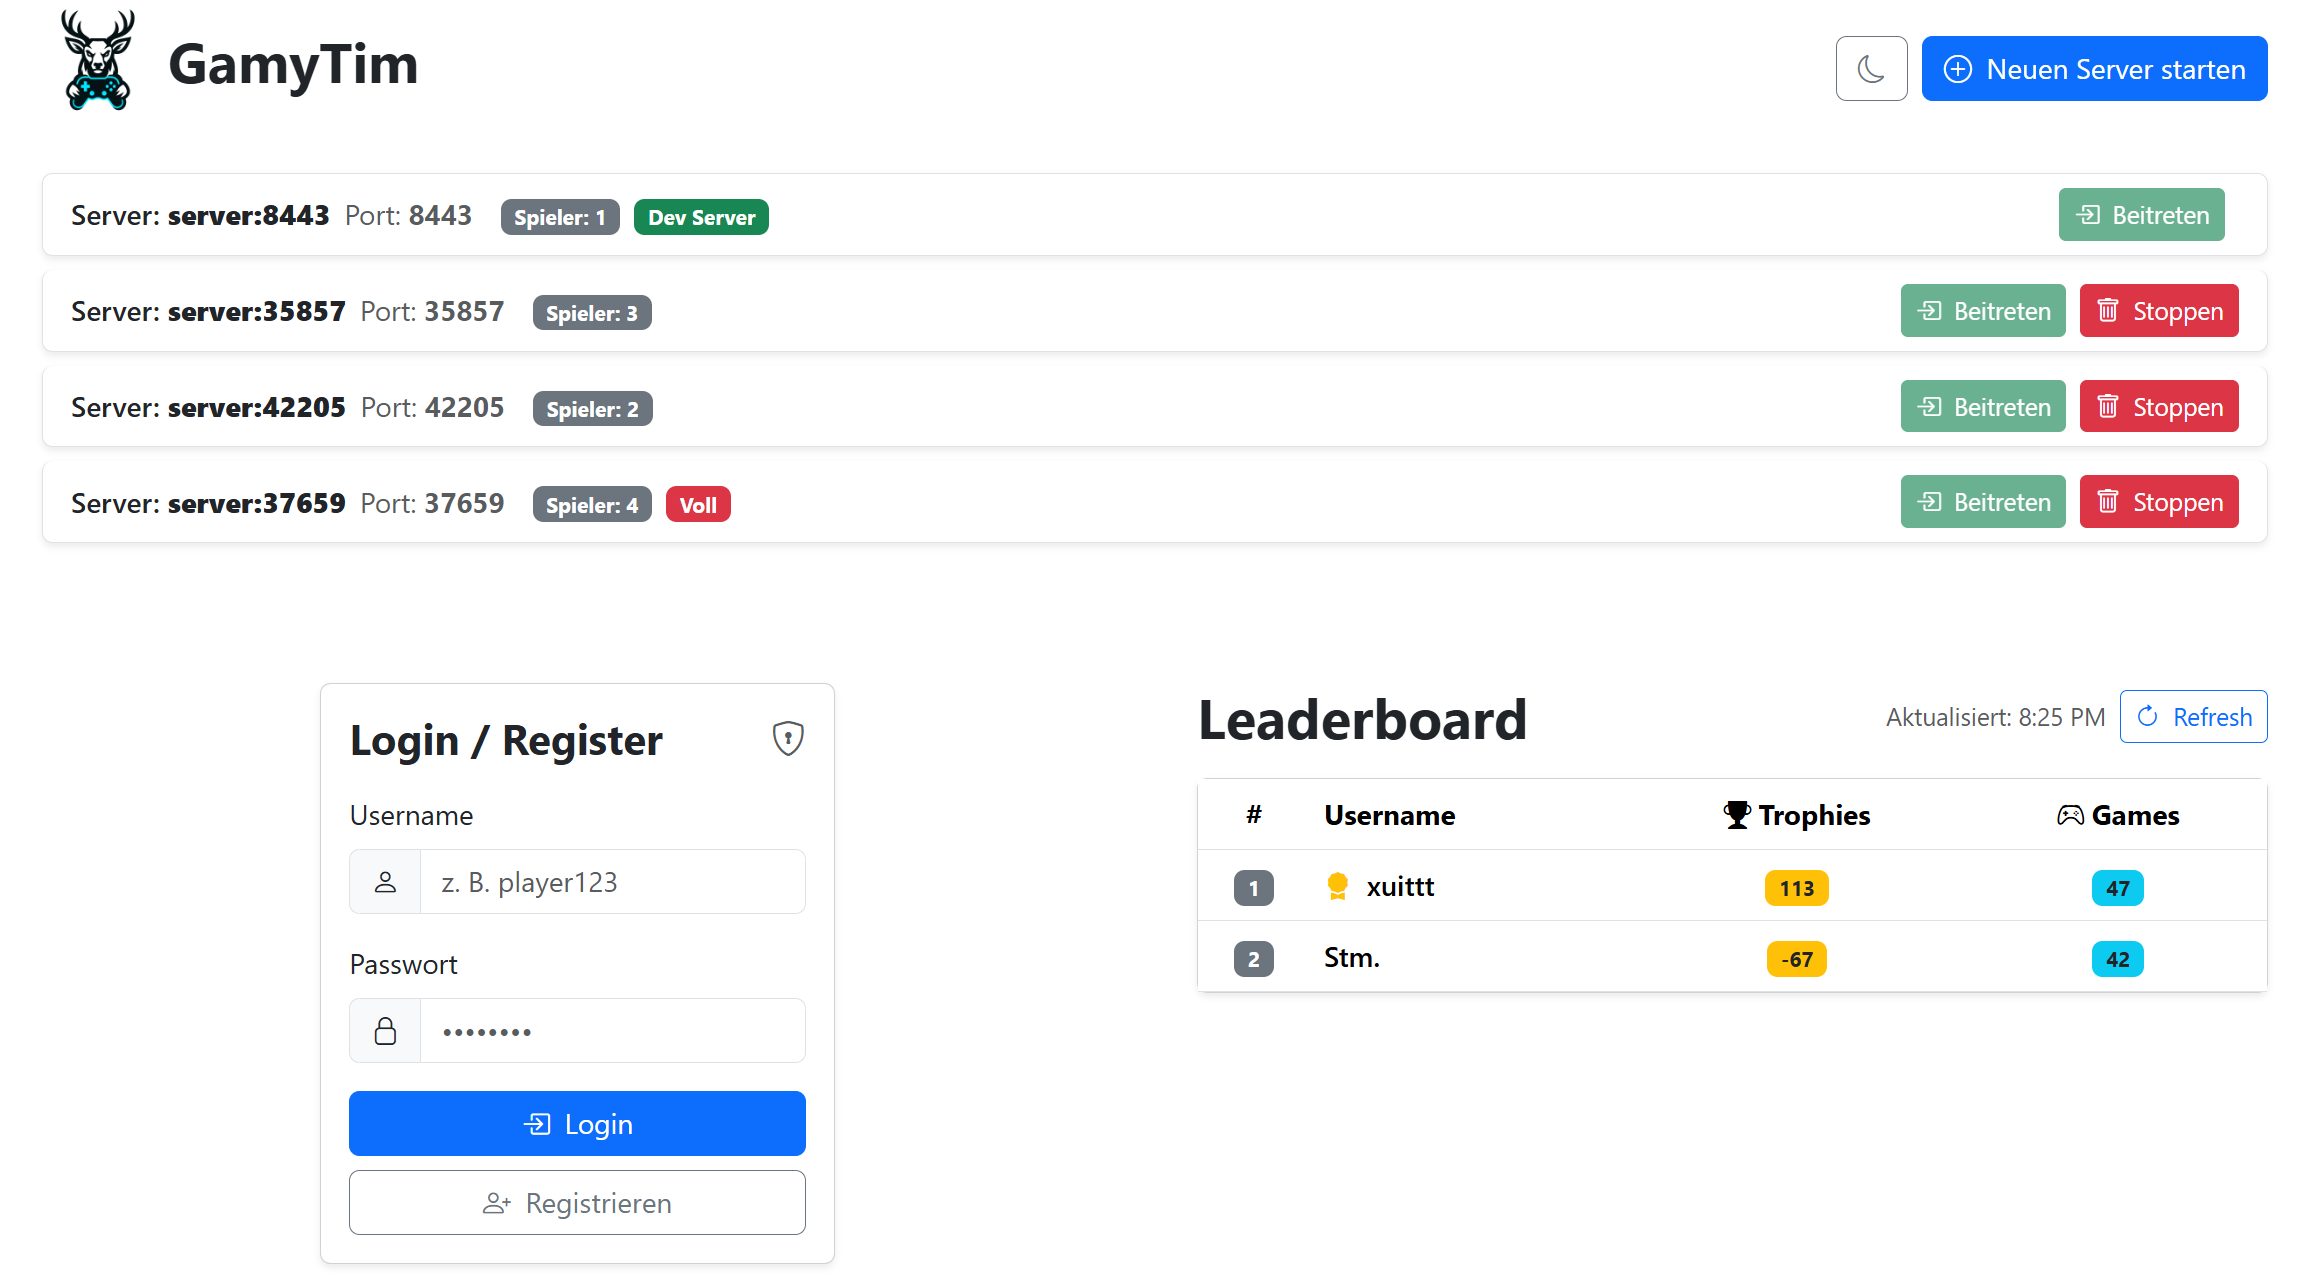
\includegraphics[width=1\linewidth]{../images/LobbyW.png}
  \caption{Frontend-Lobby des Projekts}
  \label{fig:frontend_lobby}
\end{figure}

\section{Funktionen der Lobby}
Die Frontend-Lobby umfasst mehrere Kernfunktionen, die jeweils mit Backend-Komponenten verknüpft sind:

\subsection{Login / Registrierung}
Über das Login-Formular können sich Benutzer mit einem bestehenden Account anmelden oder einen neuen Benutzer registrieren.  
Die Eingaben werden an die \textbf{UserDB} weitergeleitet, wo Validierung und Speicherung der Daten erfolgen.  
Nach erfolgreicher Anmeldung stehen dem Benutzer alle Funktionen der Lobby zur Verfügung.
\subsection{Token basierte Authentifizierung}*
Im Projekt wird die Authentifizierung über JWT umgesetzt.
Benutzer registrieren sich oder loggen sich ein, Passwörter werden mit bcrypt gehasht gespeichert.
Nach erfolgreichem Login erhält der Client ein Token, das bei allen Anfragen im Header mitgeschickt und vom Backend validiert wird.
Dadurch wird die Integrität der Benutzer-, Spiel- und Trophäendaten gewährleistet.
Um sich im GodotSpiel zu authentifizieren, wird das Token im URL-Parameter \texttt{token} übergeben, wodurch sicher gestellt wird, dass in Godot immer der Name sowie die Authorität des Spieler bekannt sind.
\noindent
Vgl. hierzu auch:  
Fettke, Peter; Vogel-Heuser, Birgit (Hrsg.): \textit{Digitale Authentifizierung und Autorisierung}, Springer Vieweg, 2021.  
Jones, M. et al.: \textit{JSON Web Token (JWT)}, IETF RFC 7519,May 2015. \url{https://datatracker.ietf.org/doc/html/rfc7519} (lezter Zugriff: 17.09.2025)

\subsection{Serverübersicht}
Im oberen Bereich wird die aktuelle Serververbindung angezeigt. 
Dabei sind \texttt{Servername}, \texttt{Port} sowie die Anzahl der verbundenen Spieler sichtbar.  
Die Daten stammen vom \textbf{Masterserver}, der kontinuierlich den Status aller verfügbaren Lobbys aktualisiert.

\subsection{Serververwaltung}
Benutzer können neue Serverinstanzen über den Button \glqq Neuen Server starten\grqq{} anlegen und ggf. bestehende Server über \glqq Stoppen\grqq{} wieder beenden.
Diese Anfrage wird an den \textbf{Loadbalancer} übermittelt, welcher die Instanz erstellt und die notwendigen Metadaten (z.\,B. Port, Lobby-ID) an den Masterserver weitergibt.

\subsection{Lobbybeitritt}
Mit der Funktion \glqq Beitreten\grqq{} können Spieler einer vorhandenen Lobby beitreten.  
Hierbei wird die Verbindung zu einem \textbf{Game-Server} hergestellt, der die eigentliche Spiellogik ausführt.  

\subsection{Leaderboard}
Das Leaderboard zeigt die globalen Punktestände und Spielstatistiken aller Spieler an.  
Die Daten werden aus der Datenbank geladen und im Frontend aktualisiert.  
Dargestellt werden unter anderem:
\begin{itemize}
  \item Benutzername,
  \item Anzahl der Trophäen,
  \item Anzahl gespielter Spiele.
  \item Leader
\end{itemize}
\subsection{Datenintegritäts-Sicherung}*
Im Backend wird über eine Validierung der einkommenden Trophäen- und Gamedaten die Integrität der Daten im Rahmen des Projektes angegangen.



\section{Godot-Spiel}
\label{chap:godot}

Das Spiel folgt dem klassischen Prinzip von \textit{Achtung, Kurve!}:  
Jeder Spieler steuert eine farbige Linie, die sich kontinuierlich über das Spielfeld bewegt.  
Ziel ist es, möglichst lange zu überleben, indem man nicht mit den Linien anderer Spieler oder den Spielfeldrändern kollidiert.  
Die Steuerung erfolgt ausschließlich über Richtungsänderungen (links/rechts).

\section{Spieloberfläche}
Die Spieloberfläche zeigt die farbigen Linien der aktiven Spieler sowie deren aktuelle Positionen (Abbildung~\ref{fig:godot_game}).  
Am oberen Rand werden die Punktestände der Spieler angezeigt, welche bei Kollisionen entsprechend angepasst werden.


\begin{figure}[h!]
  \centering
  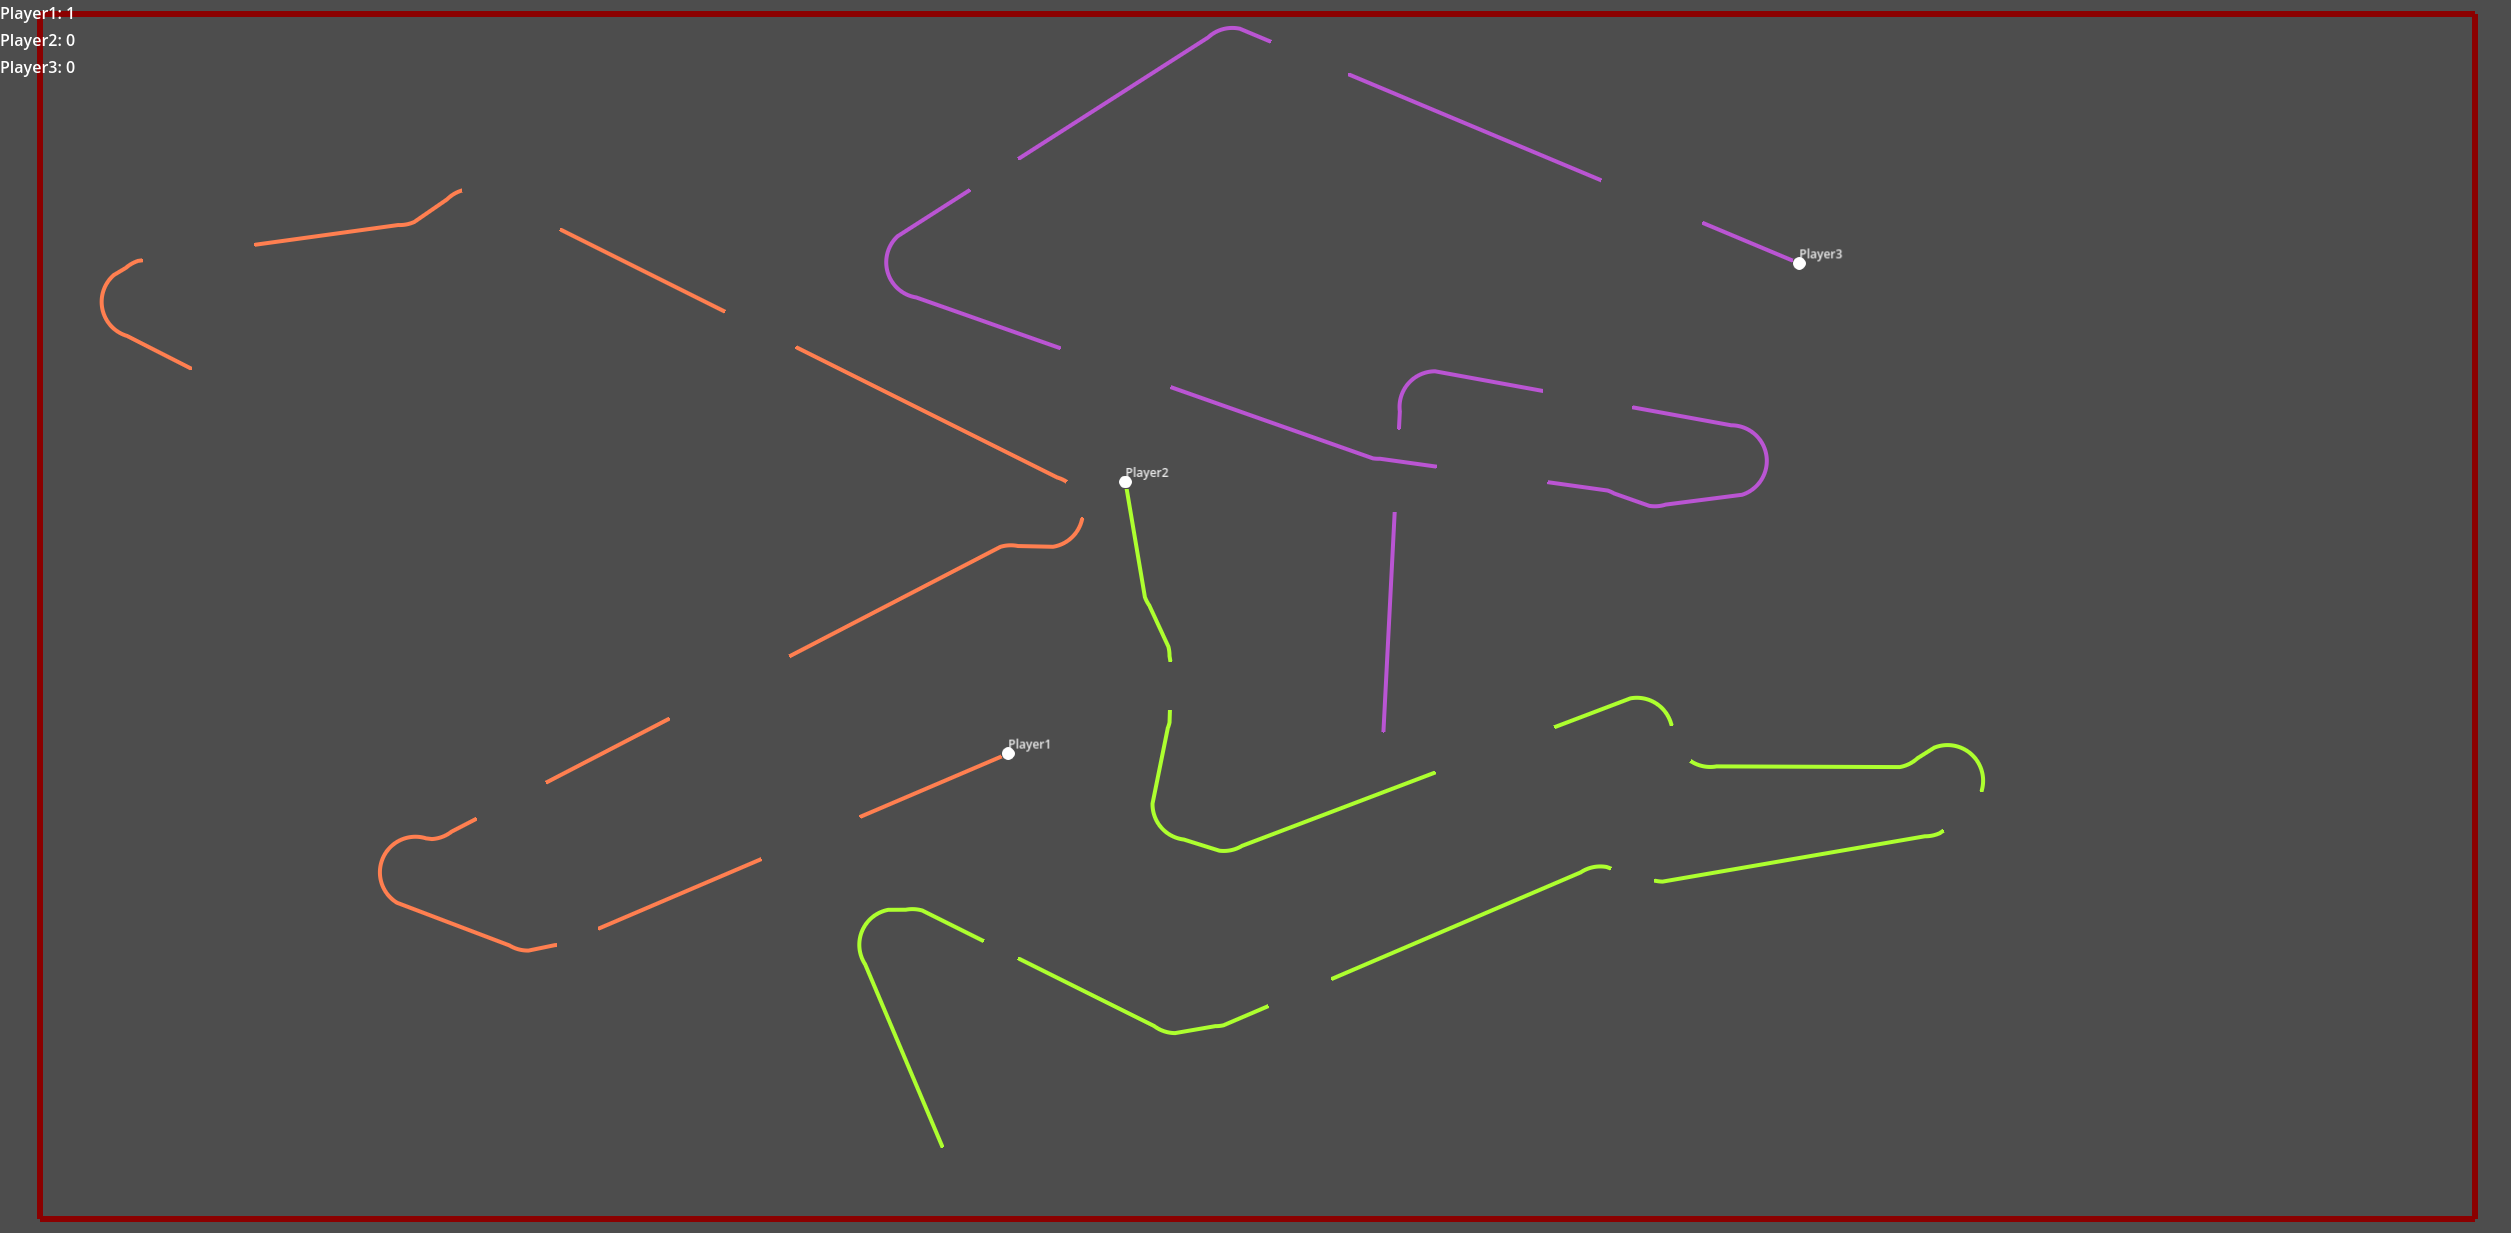
\includegraphics[width=1\linewidth]{../images/game.png}
  \caption{Spielfeld in Godot mit drei aktiven Spielern}
  \label{fig:godot_game}
\end{figure}
 
\newpage
\section{Lobby- und Ready-System}
Vor Spielbeginn wird eine Lobby-Ansicht geladen, in der sich alle Spieler sammeln.  
Hierbei übernimmt der erste Spieler die Rolle des \textbf{Hosts}.  
Alle weiteren Spieler treten über die Lobby bei.  
Jeder Spieler muss seinen Status auf \textit{Ready} setzen, bevor das Spiel starten kann.  
Die Synchronisation erfolgt über den Game-Server, der den Status aller Spieler an die Lobby zurückmeldet (Abbildung~\ref{fig:ready_system}).

\begin{figure}[h!]
  \centering
  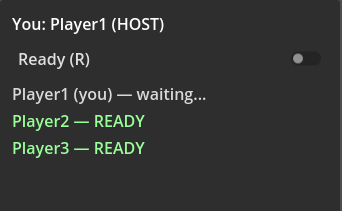
\includegraphics[width=0.4\linewidth]{../images/ready.png}
  \caption{Ready-System: alle Spieler müssen bereit sein, bevor das Spiel startet}
  \label{fig:ready_system}
\end{figure}

\noindent
Vgl. hierzu auch:  
Godot Engine Documentation: \textit{High-level multiplayer} und \textit{Networking fundamentals},  
\url{https://docs.godotengine.org/en/stable/tutorials/networking/high_level_multiplayer.html} (lezter Zugriff: 17.09.2025).  


\section{Synchronisation und Kommunikation}
Die Game-Server sind für die Synchronisation der Spiellogik verantwortlich.  
Dabei werden folgende Informationen zwischen den Instanzen ausgetauscht:
\begin{itemize}
  \item Spielerpositionen und Bewegungsrichtungen,
  \item Statusänderungen (z.\,B. Ready/Not Ready, Spielstart, Spielende),
  \item Kollisionsereignisse und daraus resultierende Punktestände.
\end{itemize}

Der zuvor bei Lobby-Beitritt festgelegte Host übernimmt die Rolle des \textbf{Master-Clients} und koordiniert die Spielabläufe.
D.h. wenn eine Kollision durch abweichende Spielabläufe auf Clientseite fälschlicherweise stattfinden, wird diese nicht erkannt. 
Nur Kollisionsereignisse, die der Master-Client erkennt, werden an alle Clients weitergegeben und somit erkannt. Dies führt zu einem geregelten Spielablauf.
Ein solches Verhalten (d.h. dass nur der Master-Client Kollisionsereignisse erkennt und propagiert) entspricht bekannten Entwurfsmustern in Multiplayer-Spielen, in denen eine autoritative Instanz (Server oder Host) nötig ist, 
um Inkonsistenzen durch etwaige Abweichungen in Client Simulationen zu vermeiden (vgl. z. B. Liljekvist, Detecting Synchronisation Problems in Networked Lockstep Games, KTH 2016; oder Artikel zu Netzwerk-Synchronisation in Multiplayer Games (lezter Zugriff: 17.09.2025) ).